% Options for packages loaded elsewhere
\PassOptionsToPackage{unicode}{hyperref}
\PassOptionsToPackage{hyphens}{url}
%
\documentclass[
]{article}
\usepackage{amsmath,amssymb}
\usepackage{lmodern}
\usepackage{iftex}
\ifPDFTeX
  \usepackage[T1]{fontenc}
  \usepackage[utf8]{inputenc}
  \usepackage{textcomp} % provide euro and other symbols
\else % if luatex or xetex
  \usepackage{unicode-math}
  \defaultfontfeatures{Scale=MatchLowercase}
  \defaultfontfeatures[\rmfamily]{Ligatures=TeX,Scale=1}
\fi
% Use upquote if available, for straight quotes in verbatim environments
\IfFileExists{upquote.sty}{\usepackage{upquote}}{}
\IfFileExists{microtype.sty}{% use microtype if available
  \usepackage[]{microtype}
  \UseMicrotypeSet[protrusion]{basicmath} % disable protrusion for tt fonts
}{}
\makeatletter
\@ifundefined{KOMAClassName}{% if non-KOMA class
  \IfFileExists{parskip.sty}{%
    \usepackage{parskip}
  }{% else
    \setlength{\parindent}{0pt}
    \setlength{\parskip}{6pt plus 2pt minus 1pt}}
}{% if KOMA class
  \KOMAoptions{parskip=half}}
\makeatother
\usepackage{xcolor}
\IfFileExists{xurl.sty}{\usepackage{xurl}}{} % add URL line breaks if available
\IfFileExists{bookmark.sty}{\usepackage{bookmark}}{\usepackage{hyperref}}
\hypersetup{
  pdftitle={Ejercicio de los carros},
  pdfauthor={Alonso Pizarro Lagunas},
  hidelinks,
  pdfcreator={LaTeX via pandoc}}
\urlstyle{same} % disable monospaced font for URLs
\usepackage[margin=1in]{geometry}
\usepackage{color}
\usepackage{fancyvrb}
\newcommand{\VerbBar}{|}
\newcommand{\VERB}{\Verb[commandchars=\\\{\}]}
\DefineVerbatimEnvironment{Highlighting}{Verbatim}{commandchars=\\\{\}}
% Add ',fontsize=\small' for more characters per line
\usepackage{framed}
\definecolor{shadecolor}{RGB}{248,248,248}
\newenvironment{Shaded}{\begin{snugshade}}{\end{snugshade}}
\newcommand{\AlertTok}[1]{\textcolor[rgb]{0.94,0.16,0.16}{#1}}
\newcommand{\AnnotationTok}[1]{\textcolor[rgb]{0.56,0.35,0.01}{\textbf{\textit{#1}}}}
\newcommand{\AttributeTok}[1]{\textcolor[rgb]{0.77,0.63,0.00}{#1}}
\newcommand{\BaseNTok}[1]{\textcolor[rgb]{0.00,0.00,0.81}{#1}}
\newcommand{\BuiltInTok}[1]{#1}
\newcommand{\CharTok}[1]{\textcolor[rgb]{0.31,0.60,0.02}{#1}}
\newcommand{\CommentTok}[1]{\textcolor[rgb]{0.56,0.35,0.01}{\textit{#1}}}
\newcommand{\CommentVarTok}[1]{\textcolor[rgb]{0.56,0.35,0.01}{\textbf{\textit{#1}}}}
\newcommand{\ConstantTok}[1]{\textcolor[rgb]{0.00,0.00,0.00}{#1}}
\newcommand{\ControlFlowTok}[1]{\textcolor[rgb]{0.13,0.29,0.53}{\textbf{#1}}}
\newcommand{\DataTypeTok}[1]{\textcolor[rgb]{0.13,0.29,0.53}{#1}}
\newcommand{\DecValTok}[1]{\textcolor[rgb]{0.00,0.00,0.81}{#1}}
\newcommand{\DocumentationTok}[1]{\textcolor[rgb]{0.56,0.35,0.01}{\textbf{\textit{#1}}}}
\newcommand{\ErrorTok}[1]{\textcolor[rgb]{0.64,0.00,0.00}{\textbf{#1}}}
\newcommand{\ExtensionTok}[1]{#1}
\newcommand{\FloatTok}[1]{\textcolor[rgb]{0.00,0.00,0.81}{#1}}
\newcommand{\FunctionTok}[1]{\textcolor[rgb]{0.00,0.00,0.00}{#1}}
\newcommand{\ImportTok}[1]{#1}
\newcommand{\InformationTok}[1]{\textcolor[rgb]{0.56,0.35,0.01}{\textbf{\textit{#1}}}}
\newcommand{\KeywordTok}[1]{\textcolor[rgb]{0.13,0.29,0.53}{\textbf{#1}}}
\newcommand{\NormalTok}[1]{#1}
\newcommand{\OperatorTok}[1]{\textcolor[rgb]{0.81,0.36,0.00}{\textbf{#1}}}
\newcommand{\OtherTok}[1]{\textcolor[rgb]{0.56,0.35,0.01}{#1}}
\newcommand{\PreprocessorTok}[1]{\textcolor[rgb]{0.56,0.35,0.01}{\textit{#1}}}
\newcommand{\RegionMarkerTok}[1]{#1}
\newcommand{\SpecialCharTok}[1]{\textcolor[rgb]{0.00,0.00,0.00}{#1}}
\newcommand{\SpecialStringTok}[1]{\textcolor[rgb]{0.31,0.60,0.02}{#1}}
\newcommand{\StringTok}[1]{\textcolor[rgb]{0.31,0.60,0.02}{#1}}
\newcommand{\VariableTok}[1]{\textcolor[rgb]{0.00,0.00,0.00}{#1}}
\newcommand{\VerbatimStringTok}[1]{\textcolor[rgb]{0.31,0.60,0.02}{#1}}
\newcommand{\WarningTok}[1]{\textcolor[rgb]{0.56,0.35,0.01}{\textbf{\textit{#1}}}}
\usepackage{graphicx}
\makeatletter
\def\maxwidth{\ifdim\Gin@nat@width>\linewidth\linewidth\else\Gin@nat@width\fi}
\def\maxheight{\ifdim\Gin@nat@height>\textheight\textheight\else\Gin@nat@height\fi}
\makeatother
% Scale images if necessary, so that they will not overflow the page
% margins by default, and it is still possible to overwrite the defaults
% using explicit options in \includegraphics[width, height, ...]{}
\setkeys{Gin}{width=\maxwidth,height=\maxheight,keepaspectratio}
% Set default figure placement to htbp
\makeatletter
\def\fps@figure{htbp}
\makeatother
\setlength{\emergencystretch}{3em} % prevent overfull lines
\providecommand{\tightlist}{%
  \setlength{\itemsep}{0pt}\setlength{\parskip}{0pt}}
\setcounter{secnumdepth}{-\maxdimen} % remove section numbering
\ifLuaTeX
  \usepackage{selnolig}  % disable illegal ligatures
\fi

\title{Ejercicio de los carros}
\author{\emph{Alonso Pizarro Lagunas}}
\date{\emph{23/12/2021}}

\begin{document}
\maketitle

\hypertarget{anuxe1lisis-de-los-coches-con-database-mtcars-de-ggplot}{%
\subsection{Análisis de los coches con database `mtcars' de
ggplot}\label{anuxe1lisis-de-los-coches-con-database-mtcars-de-ggplot}}

\begin{Shaded}
\begin{Highlighting}[]
\FunctionTok{library}\NormalTok{(ggplot2)}
\NormalTok{mtcars }\OtherTok{\textless{}{-}}\NormalTok{  mtcars}
\end{Highlighting}
\end{Shaded}

\hypertarget{carga-de-datos-en-python.}{%
\subsubsection{\texorpdfstring{Carga de datos en
\texttt{Python}.}{Carga de datos en Python.}}\label{carga-de-datos-en-python.}}

\begin{Shaded}
\begin{Highlighting}[]
\ImportTok{import}\NormalTok{ pandas }\ImportTok{as}\NormalTok{ pd     }\CommentTok{\# Pandas}
\ImportTok{import}\NormalTok{ numpy  }\ImportTok{as}\NormalTok{ np     }\CommentTok{\# Numpy }
\ImportTok{import}\NormalTok{ matplotlib.pyplot }\ImportTok{as}\NormalTok{ plt  }\CommentTok{\# Matplotlib }


\NormalTok{mtcars }\OperatorTok{=}\NormalTok{ r.mtcars       }\CommentTok{\# El DF que se cargo desde R ahora lo cargamos en python }
\BuiltInTok{print}\NormalTok{(mtcars.shape)     }\CommentTok{\# Vemos la dimensión de nuestra data }
\end{Highlighting}
\end{Shaded}

\begin{verbatim}
## (32, 11)
\end{verbatim}

\begin{Shaded}
\begin{Highlighting}[]
\BuiltInTok{print}\NormalTok{(mtcars.head())    }\CommentTok{\# Visualizamos las primeras líneas de data}
\end{Highlighting}
\end{Shaded}

\begin{verbatim}
##                     mpg  cyl   disp     hp  drat  ...   qsec   vs   am  gear  carb
## Mazda RX4          21.0  6.0  160.0  110.0  3.90  ...  16.46  0.0  1.0   4.0   4.0
## Mazda RX4 Wag      21.0  6.0  160.0  110.0  3.90  ...  17.02  0.0  1.0   4.0   4.0
## Datsun 710         22.8  4.0  108.0   93.0  3.85  ...  18.61  1.0  1.0   4.0   1.0
## Hornet 4 Drive     21.4  6.0  258.0  110.0  3.08  ...  19.44  1.0  0.0   3.0   1.0
## Hornet Sportabout  18.7  8.0  360.0  175.0  3.15  ...  17.02  0.0  0.0   3.0   2.0
## 
## [5 rows x 11 columns]
\end{verbatim}

\hypertarget{medidas-de-centralizaciuxf3n}{%
\subsubsection{Medidas de
Centralización}\label{medidas-de-centralizaciuxf3n}}

\begin{Shaded}
\begin{Highlighting}[]
\BuiltInTok{print}\NormalTok{(mtcars.mean())    }\CommentTok{\# Media de cada una de las columnas}
\end{Highlighting}
\end{Shaded}

\begin{verbatim}
## mpg      20.090625
## cyl       6.187500
## disp    230.721875
## hp      146.687500
## drat      3.596563
## wt        3.217250
## qsec     17.848750
## vs        0.437500
## am        0.406250
## gear      3.687500
## carb      2.812500
## dtype: float64
\end{verbatim}

\begin{Shaded}
\begin{Highlighting}[]
\BuiltInTok{print}\NormalTok{(mtcars.mean(axis }\OperatorTok{=} \DecValTok{1}\NormalTok{))  }\CommentTok{\# Media por filas (Nota que esto no hace mucho sentido)}
\end{Highlighting}
\end{Shaded}

\begin{verbatim}
## Mazda RX4              29.907273
## Mazda RX4 Wag          29.981364
## Datsun 710             23.598182
## Hornet 4 Drive         38.739545
## Hornet Sportabout      53.664545
## Valiant                35.049091
## Duster 360             59.720000
## Merc 240D              24.634545
## Merc 230               27.233636
## Merc 280               31.860000
## Merc 280C              31.787273
## Merc 450SE             46.430909
## Merc 450SL             46.500000
## Merc 450SLC            46.350000
## Cadillac Fleetwood     66.232727
## Lincoln Continental    66.058545
## Chrysler Imperial      65.972273
## Fiat 128               19.440909
## Honda Civic            17.742273
## Toyota Corolla         18.814091
## Toyota Corona          24.888636
## Dodge Challenger       47.240909
## AMC Javelin            46.007727
## Camaro Z28             58.752727
## Pontiac Firebird       57.379545
## Fiat X1-9              18.928636
## Porsche 914-2          24.779091
## Lotus Europa           24.880273
## Ford Pantera L         60.971818
## Ferrari Dino           34.508182
## Maserati Bora          63.155455
## Volvo 142E             26.262727
## dtype: float64
\end{verbatim}

\begin{Shaded}
\begin{Highlighting}[]
\BuiltInTok{print}\NormalTok{(mtcars.median()) }\CommentTok{\# Mediana para cada una de las columnas}
\end{Highlighting}
\end{Shaded}

\begin{verbatim}
## mpg      19.200
## cyl       6.000
## disp    196.300
## hp      123.000
## drat      3.695
## wt        3.325
## qsec     17.710
## vs        0.000
## am        0.000
## gear      4.000
## carb      2.000
## dtype: float64
\end{verbatim}

\begin{Shaded}
\begin{Highlighting}[]
\BuiltInTok{print}\NormalTok{(mtcars[}\StringTok{\textquotesingle{}mpg\textquotesingle{}}\NormalTok{].mean()) }\CommentTok{\# media para la columna de \textquotesingle{}mpg\textquotesingle{}}
\end{Highlighting}
\end{Shaded}

\begin{verbatim}
## 20.090624999999996
\end{verbatim}

\hypertarget{medidas-contra-distribuciones}{%
\subsubsection{Medidas contra
distribuciones}\label{medidas-contra-distribuciones}}

\begin{Shaded}
\begin{Highlighting}[]
\NormalTok{normData }\OperatorTok{=}\NormalTok{ pd.DataFrame(np.random.normal(size}\OperatorTok{=}\DecValTok{100000}\NormalTok{)) }\CommentTok{\# Generamos datos normalmente dist.}

\NormalTok{normData.plot(kind }\OperatorTok{=} \StringTok{\textquotesingle{}density\textquotesingle{}}\NormalTok{, figsize}\OperatorTok{=}\NormalTok{(}\DecValTok{10}\NormalTok{,}\DecValTok{10}\NormalTok{)) }\CommentTok{\# Grafica}
\NormalTok{plt.vlines(normData.mean(), ymin }\OperatorTok{=} \DecValTok{0}\NormalTok{, ymax }\OperatorTok{=} \FloatTok{0.4}\NormalTok{,}
\NormalTok{linewidth}\OperatorTok{=}\FloatTok{5.0}\NormalTok{, color }\OperatorTok{=} \StringTok{"blue"}\NormalTok{)}
\NormalTok{plt.vlines(normData.median(), ymin }\OperatorTok{=} \DecValTok{0}\NormalTok{, ymax }\OperatorTok{=} \FloatTok{0.4}\NormalTok{,}
\NormalTok{linewidth}\OperatorTok{=}\FloatTok{2.5}\NormalTok{, color }\OperatorTok{=} \StringTok{"red"}\NormalTok{)}
\NormalTok{plt.title(}\StringTok{\textquotesingle{}Distribucion normal\textquotesingle{}}\NormalTok{)}
\NormalTok{plt.show()}
\end{Highlighting}
\end{Shaded}

\begin{center}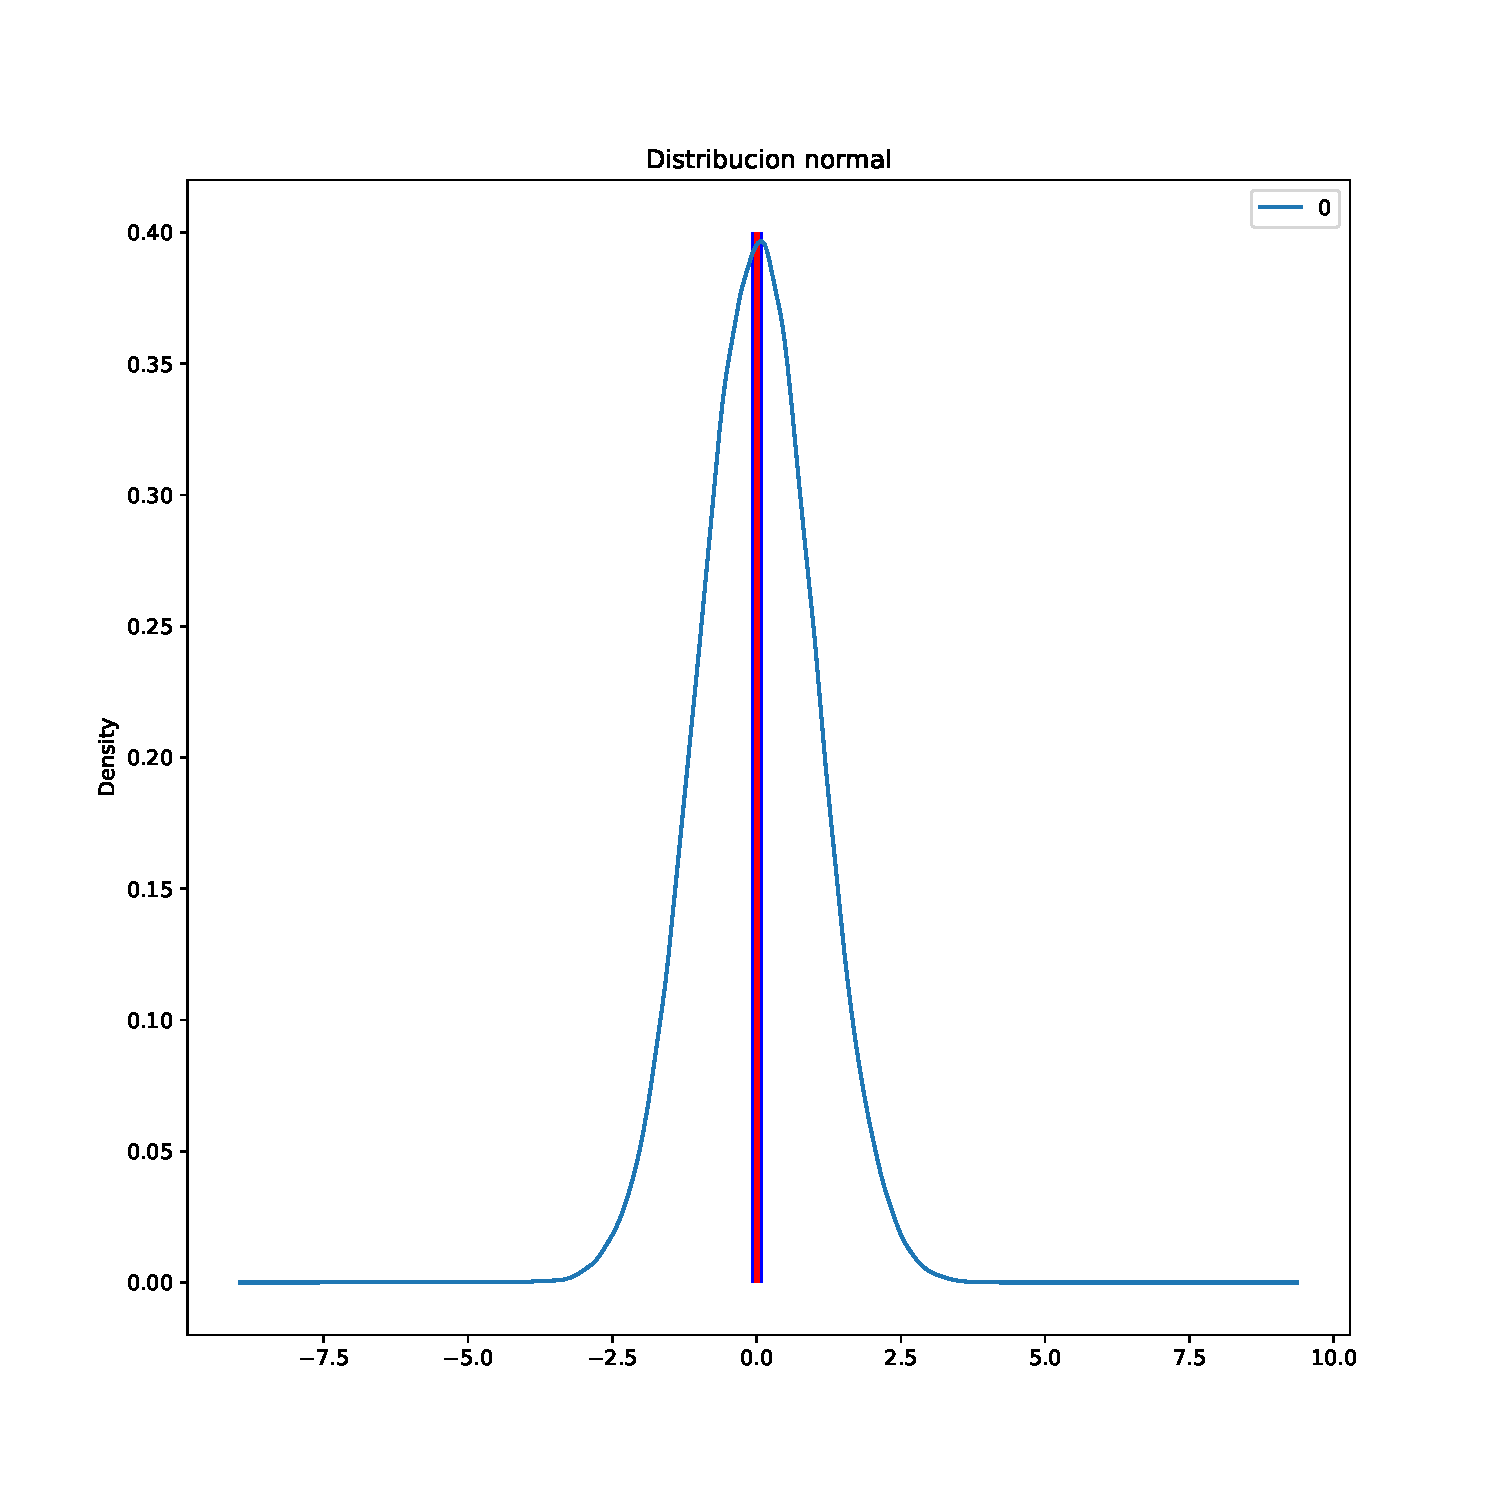
\includegraphics{Ejercicio-de-los-Carros_files/figure-latex/unnamed-chunk-4-1} \end{center}

\hypertarget{muestras-con-sesgos}{%
\subsubsection{Muestras con sesgos}\label{muestras-con-sesgos}}

\begin{Shaded}
\begin{Highlighting}[]
\NormalTok{skewedData }\OperatorTok{=}\NormalTok{ pd.DataFrame(np.random.exponential(size}\OperatorTok{=}\DecValTok{100000}\NormalTok{)) }\CommentTok{\# Generamos datos normalmente dist.}

\NormalTok{skewedData.plot(kind }\OperatorTok{=} \StringTok{\textquotesingle{}density\textquotesingle{}}\NormalTok{, figsize}\OperatorTok{=}\NormalTok{(}\DecValTok{10}\NormalTok{,}\DecValTok{10}\NormalTok{), xlim }\OperatorTok{=}\NormalTok{ (}\OperatorTok{{-}}\DecValTok{1}\NormalTok{,}\DecValTok{5}\NormalTok{)) }\CommentTok{\# Grafica}
\NormalTok{plt.vlines(skewedData.mean(), ymin }\OperatorTok{=} \DecValTok{0}\NormalTok{, ymax }\OperatorTok{=} \FloatTok{1.0}\NormalTok{,}
\NormalTok{linewidth}\OperatorTok{=}\FloatTok{5.0}\NormalTok{, color }\OperatorTok{=} \StringTok{"blue"}\NormalTok{)}
\NormalTok{plt.vlines(skewedData.median(), ymin }\OperatorTok{=} \DecValTok{0}\NormalTok{, ymax }\OperatorTok{=} \FloatTok{1.0}\NormalTok{,}
\NormalTok{linewidth}\OperatorTok{=}\FloatTok{2.5}\NormalTok{, color }\OperatorTok{=} \StringTok{"red"}\NormalTok{)}
\NormalTok{plt.title(}\StringTok{\textquotesingle{}Distribucion sesgada\textquotesingle{}}\NormalTok{)}
\NormalTok{plt.show()}
\end{Highlighting}
\end{Shaded}

\begin{center}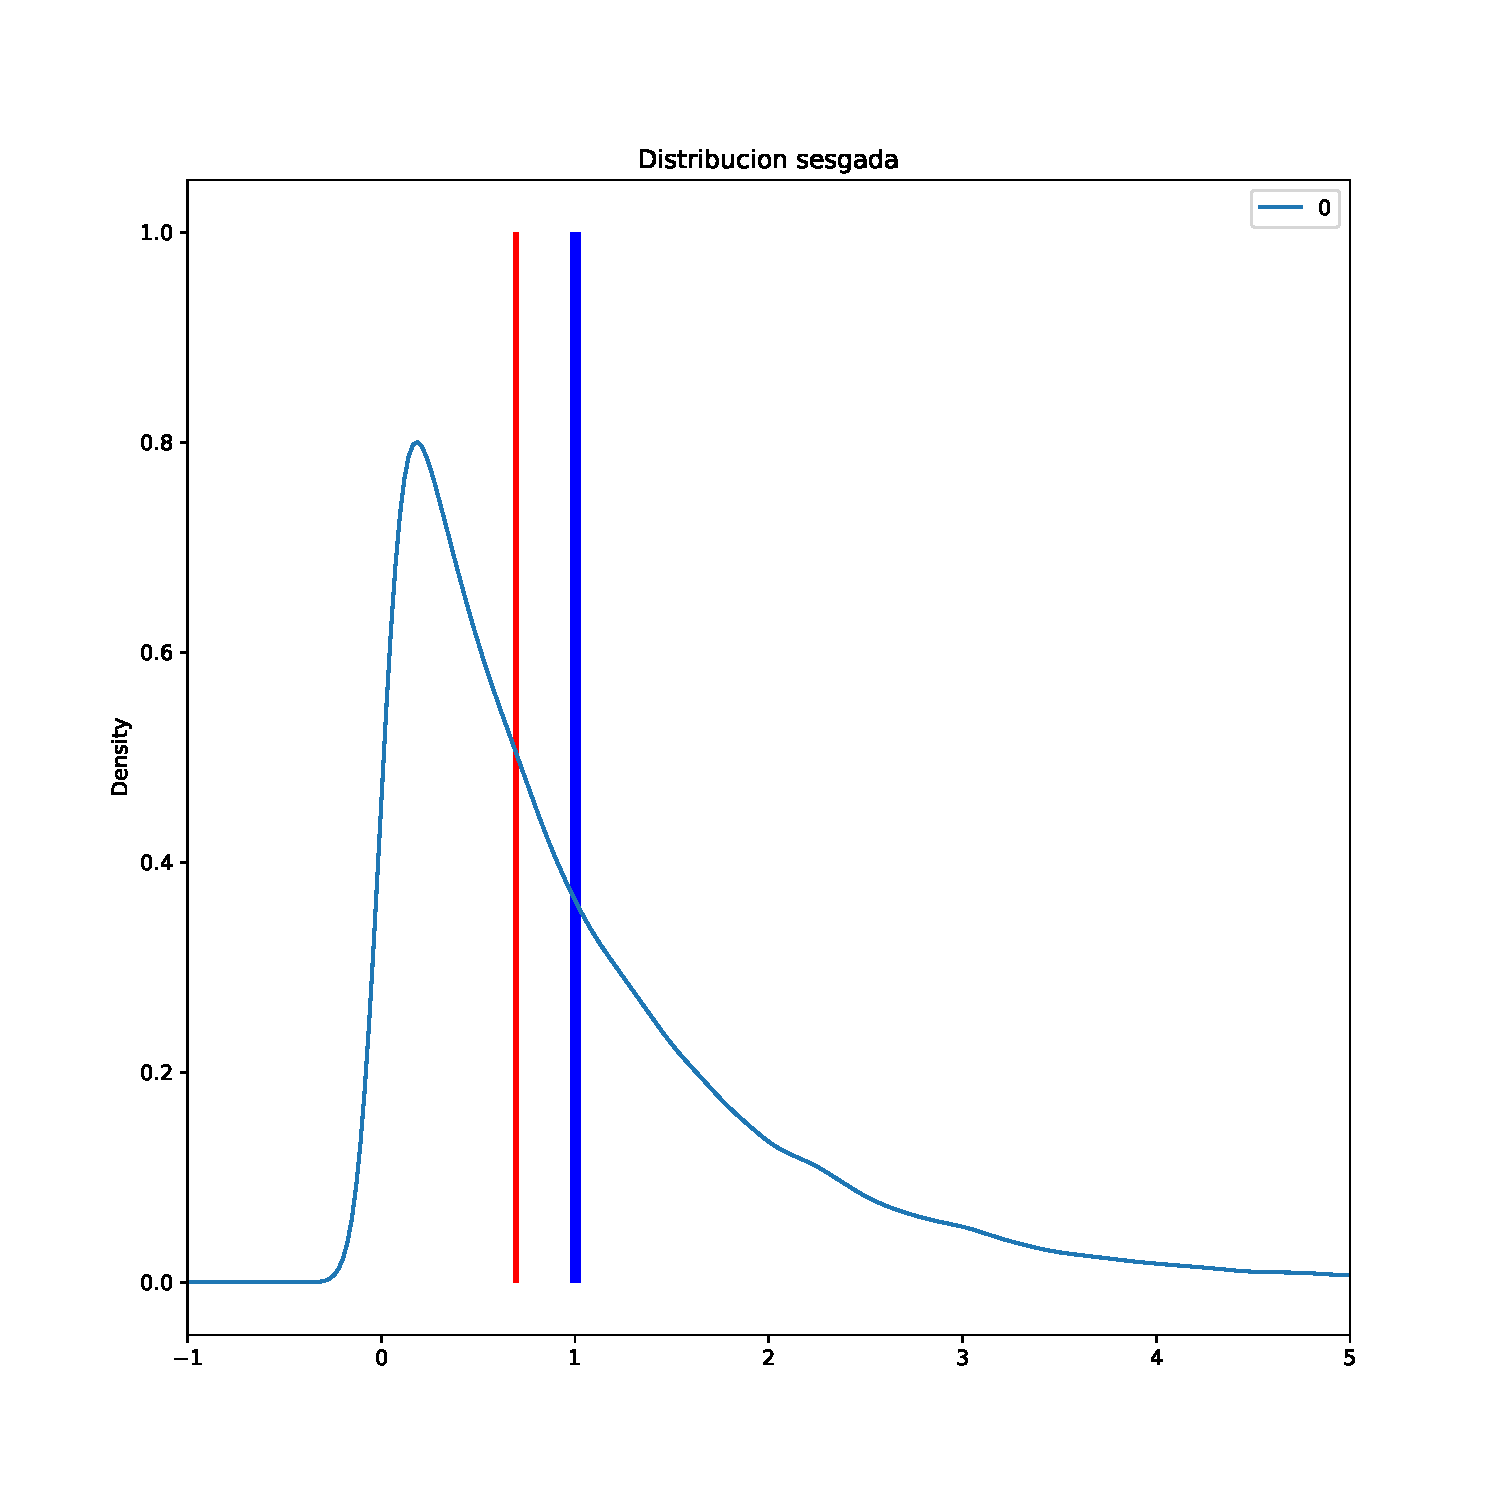
\includegraphics{Ejercicio-de-los-Carros_files/figure-latex/unnamed-chunk-5-3} \end{center}

\end{document}
